%%%%%%%%%%%%%%%%%%%%%%% file template.tex %%%%%%%%%%%%%%%%%%%%%%%%%
%
% This is a general template file for the LaTeX package SVJour3
% for Springer journals.          Springer Heidelberg 2010/09/16
%
% Copy it to a new file with a new name and use it as the basis
% for your article. Delete % signs as needed.
%
% This template includes a few options for different layouts and
% content for various journals. Please consult a previous issue of
% your journal as needed.
%
%%%%%%%%%%%%%%%%%%%%%%%%%%%%%%%%%%%%%%%%%%%%%%%%%%%%%%%%%%%%%%%%%%%
%
% First comes an example EPS file -- just ignore it and
% proceed on the \documentclass line
% your LaTeX will extract the file if required
% \begin{filecontents*}{example.eps}
% %!PS-Adobe-3.0 EPSF-3.0
% %%BoundingBox: 19 19 221 221
% %%CreationDate: Mon Sep 29 1997
% %%Creator: programmed by hand (JK)
% %%EndComments
% gsave
% newpath
%   20 20 moveto
%   20 220 lineto
%   220 220 lineto
%   220 20 lineto
% closepath
% 2 setlinewidth
% gsave
%   .4 setgray fill
% grestore
% stroke
% grestore
% \end{filecontents*}
%
\RequirePackage{fix-cm}
%
\documentclass{svjour3}                     % onecolumn (standard format)
%\documentclass[smallcondensed]{svjour3}     % onecolumn (ditto)
%\documentclass[smallextended]{svjour3}       % onecolumn (second format)
%\documentclass[twocolumn]{svjour3}          % twocolumn
%
\smartqed  % flush right qed marks, e.g. at end of proof

\usepackage{graphicx}
\usepackage{ragged2e}

\usepackage{mathptmx}      % use Times fonts if available on your TeX system
\usepackage{amsfonts}
\usepackage{amsmath}
\usepackage{amssymb}
\usepackage{cite}
\usepackage[section]{placeins}
\usepackage{multirow}
\usepackage{bigstrut}

\usepackage{caption}
\captionsetup{justification=centering}
%
% insert here the call for the packages your document requires
%\usepackage{latexsym}
% etc.
%
% please place your own definitions here and don't use \def but
% \newcommand{}{}
%
% Insert the name of "your journal" with
\journalname{International Journal of Information Technology}
%

\begin{document}
\notag
\sloppy
\hbadness=10001
\vbadness=10001
\title{MES\,$-$\,Modern Encryption Standard%\thanks{Grants or other notes
%about the article that should go on the front page should be
%placed here. General acknowledgments should be placed at the end of the article.}
}
%\subtitle{Do you have a subtitle?\\ If so, write it here}

%\titlerunning{Short form of title}        % if too long for running head

\author{Awnon Bhowmik \and
        Unnikrishnan Menon %etc.
}

%\authorrunning{Short form of author list} % if too long for running head

\institute{Awnon Bhowmik \at Department of Mathematics \& Computer Science, CUNY York College, USA\\
              90\,$-$\,24 Guy R. Brewer Blvd, Jamaica, NY 11451\\
              %Tel.: +929-462-8832\\
              %Fax: +123-45-678910\\
              \email{awnon.bhowmik@yorkmail.cuny.edu}           %  \\
%             \emph{Present address:} of F. Author  %  if needed
           \and
           Unnikrishnan Menon \at Department of Electrical and Electronics Engineering, Vellore Institute of Technology\\
           Vellore, Tamil Nadu 632014, India\\
           \email{unnikrishnanr.menon2017@vitstudent.ac.in}
}

\date{Received: date / Accepted: date}
% The correct dates will be entered by the editor


\maketitle

\begin{abstract}
As mathematical theory has evolved and computing capabilities have improved, what initially seemed to be adequately difficult trapdoor functions, were deemed not to be later on. In this paper, a new block-encryption scheme named Modern Encryption Standard (MES) is proposed based on the multiple concepts arising from number theory for a highly secure and fast cryptosystem that can be considered as an alternative to the existing systems. This is a block cipher like AES, but the inherent algorithm is quite different. The security of the proposed MES algorithm stands on the fundamentals of the Chinese Remainder Theorem, Cantor Pairing Function and the Prime Number Theorem for creating an ingenious trapdoor function. Breaking this algorithm proves to be quite a daunting obstacle to overcome for an unwelcome interceptor.
\keywords{AES \and DES \and NIST \and MES \and modern encryption \and Modern Encryption Standard \and 3DES \and Triple DES \and Chinese Remainder Theorem \and Cantor Pairing Function \and Shor's Algorithm \and Pollard's Rho Algorithm}
% \PACS{PACS code1 \and PACS code2 \and more}
% \subclass{MSC code1 \and MSC code2 \and more}
\end{abstract}

\newpage
\section{Introduction}
\label{intro}
In July 2017, National Institute of Standards and Technology (NIST) initially proposed retiring Triple Data Encryption Standard (3DES) following a security analysis and practical demonstration of attacks on 3DES in several real-world protocols. In November 2017, NIST restricted usage to 220 64-bit blocks (8 MB of data) using a single key bundle, so it could no longer effectively be used for TLS, IPsec, or large file encryption.

Advanced Encryption Standard (AES) was introduced in 2001 to replace 3DES. Data Encryption Standard (DES), the algorithm is based on, was retired in 2005. NIST is supposedly going to retire 3DES by 2023, leaving only AES as the strongest candidate to be widely used in all of hardware and software security protocols. Owing to the research and rapid developments in the sector of cryptanalysis, modern cryptographers are posed with the constant challenge to develop superior cryptosystems so that it takes an interceptor to spend a certain period in the system which allows the concerned authorities to track them down. This means they must be able to develop enigmatic trapdoor functions in order to achieve this.

\section{Trapdoor Function}
\label{sec:2}
\begin{flushleft}
A trapdoor function is a highly useful concept in modern cryptography. These are functions that are easy to compute in one direction but extremely hard to compute in reverse if certain parameters or critical information for reversal is lacked. The main novelty of this cryptosystem is the use of the fundamental Chinese Remainder Theorem as a trapdoor function. The algorithm starts off with a secret message that needs to be encrypted (called the plainText).
\end{flushleft}

\section{Chinese Remainder Theorem}
\label{sec:3}
\paragraph{Statement:} Let $m_1,m_2,\cdots,m_n$ be $n$ arbitrary integers. If all $n_i$'s are pairwise co-prime, and if $a_1,a_2,\cdots,a_n$ are integers such that $0\le a_i<m_i$ for every $i$, then there is one and only one $x$ such that
    \begin{align}
        x&\equiv a_1\mod m_1\\
        x&\equiv a_2\mod m_2\\
        \vdots\\
        x&\equiv a_n\mod m_n
    \end{align}
The solution is given by $$x\equiv k\text{ lcm}(m_1,m_2,\cdots,m_n)$$
This theorem implies we can represent an element of $\mathbb{Z}_{pq}$ by one element of $\mathbb{Z}_p$ and one element of $\mathbb{Z}_q$, and vice versa. In other words, we have a bijection between $\mathbb{Z_{pq}}$ and $\mathbb{Z}_p\times\mathbb{Z}_q$.

\subsection{Direct Construction}
The computational steps for Chinese Remainder Theorem is as follows
\begin{enumerate}
    \item Compute $M=\text{lcm}(m_1m_2\cdots m_n)$
    \item Let $M_i=\dfrac{M}{m_i}$ be the product of all moduli but one. Since $m_i$'s are pairwise co-prime, $M_i$ and $m_i$ are co-prime.
    \item Applying \textit{Bezout's Theorem}, there exists integers $K_i$ and $k_i$ such that $$K_iM_i+k_im_i=1$$
    \item Then the solution is given by $$x=\sum_{i=1}^na_iM_iK_i$$
\end{enumerate}
There has been numerous papers \cite{number_theory_the_chinese_remainder_theorem,dingyi1996chinese,douguet2012chinese,grossschadl2000chinese,wu2001rsa} where the authors have used Chinese Remainder Theorem to generate a private key or to encrypt a given message. It usually involved finding a solution for a set of two simultaneous congruence relations. This paper involves finding a solution to a set of two or many more such equations and a unique key generation paradigm based on the prime number theorem.
\section{Cantor Pairing Function}
\label{sec:4}
This is an elegant function proposed by the Russian mathematician George Cantor that takes in two natural numbers and turns it into a single number. This function is a primitive recursive pairing function. $$C:\mathbb{N}\times\mathbb{N}\to\mathbb{N}$$
and is defined by $$C(x,y)=\dfrac12(x+y)(x+y+1)+y$$
Due to the way its defined, this is a one-to-one and onto function, which means it is invertible. This consequently means that given a single number, it can be readily mapped back to a unique $(x,y)$ ordered pair. In order to retrieve an ordered pair $(x,y)$ from a given $t$, the following transformations are used
    \begin{align*}
        \omega&=x+y\\
        t&=\dfrac12\omega(\omega+1)
    \end{align*}
From the second equation, cross multiplying gives a quadratic in $\omega$
$$\omega^2+\omega-2t=0$$
Solving it gives us
$$\omega=\dfrac{\sqrt{8t+1}-1}{2}$$
which is a strictly increasing and continuous function when $t$ is non-negative real. Since $$t\le z=t+y<t+(\omega+1)=\dfrac{(\omega+1)^2+(\omega+1)}2$$
This implies that
$$\omega\le\dfrac{\sqrt{8z+1}-1}2<\omega+1$$
And thus
$$\omega=\left\lfloor\dfrac{\sqrt{8z+1}-1}2\right\rfloor$$
Finally calculate $x$ and $y$ from $z$ as follows
    \begin{align*}
        \omega&=\left\lfloor\dfrac{\sqrt{8z+1}-1}2\right\rfloor\\
        t&=\dfrac12\omega(\omega+1)\\
        y&=z-t\\
        x&=\omega-y
    \end{align*}

\FloatBarrier
\section{Prime number theorem}
\label{sec:5}
Positive integers that are divisible by $1$ and itself, are known as \textit{prime numbers}. The sequence begins like the following... $$2, 3, 5, 7, 11, 13, 17, 19, 23, 29, 31, 37, \cdots$$ has held untold fascination for mathematicians, both professionals and amateurs alike. A result that gives an idea about an asymptotic distribution of primes is known as the \textit{prime number theorem} \cite{goldstein1973history}.

Let $\pi(x)$ be the prime-counting function that gives the number of primes less than or equal to $x$, for any real number $x$. For example, $\pi(10) = 4$ because there are four prime numbers $(2, 3, 5 \text{ and } 7)$ less than or equal to $10$. The prime number theorem then states that $\dfrac{x}{\ln x}$ is a good approximation to $\pi(x)$, in the sense that the limit of the quotient of the two functions $\pi(x)$ and $\dfrac{x}{\ln x}$ as $x$ increases without bound is 1 $$\lim_{x\to\infty}\pi(x)\dfrac{\ln x}{x}=1$$ known as the asymptotic law of distribution of prime numbers. Using asymptotic notation this result can be restated as $$\pi(x)\sim\dfrac{x}{\ln x}$$

The \textit{logarithmic integral} provides a good estimate to the prime counting function.$$\pi(x)\sim \operatorname{li}(x)$$

In order to get an idea of the distribution of primes, it is important to count the number of primes in a given range and find the percentage of primes. The following table demonstrates this.

\begin{table}[htbp!]
% table caption is above the table
\caption{Prime density and approximation to logarithmic integral}
\label{tab:1}       % Give a unique label
\centering
    % For LaTeX tables use
\begin{tabular}{c|r|r|r|c}
\hline\noalign{\smallskip}
Search Size $x$& \# of primes & Density (\%) & $\operatorname{li}(x)$ & $\dfrac{\operatorname{li}(x)-\pi(x)}{\pi(x)}\times 100\%$\\
\noalign{\smallskip}\hline\noalign{\smallskip}
$10$ & $4$ & $40$ & $6.16$ & $54.14$\\
$10^2$ & $25$ & $25$ & $30.13$ & $20.50$\\
$10^3$ & $168$ & $16.8$ & $177.61$ & $5.72$\\
$10^4$ & $1229$ & $12.3$ & $1246.14$ & $1.39$\\
$10^5$ & $9592$ & $9.6$ & $9629.81$ & $0.39$\\
$10^6$ & $78498$ & $7.8$ & $78625$ & $0.17$\\
$10^7$ & $664579$ & $6.6$ & $664918$ & $0.05$\\
$10^8$ & $5761455$ & $5.8$ & $5.76\times 10^6$ & $0.01$\\
\noalign{\smallskip}\hline
\end{tabular}
\end{table}

\FloatBarrier
Following is a visual demonstration.

    \begin{figure*}[hbt!]
        \centering
        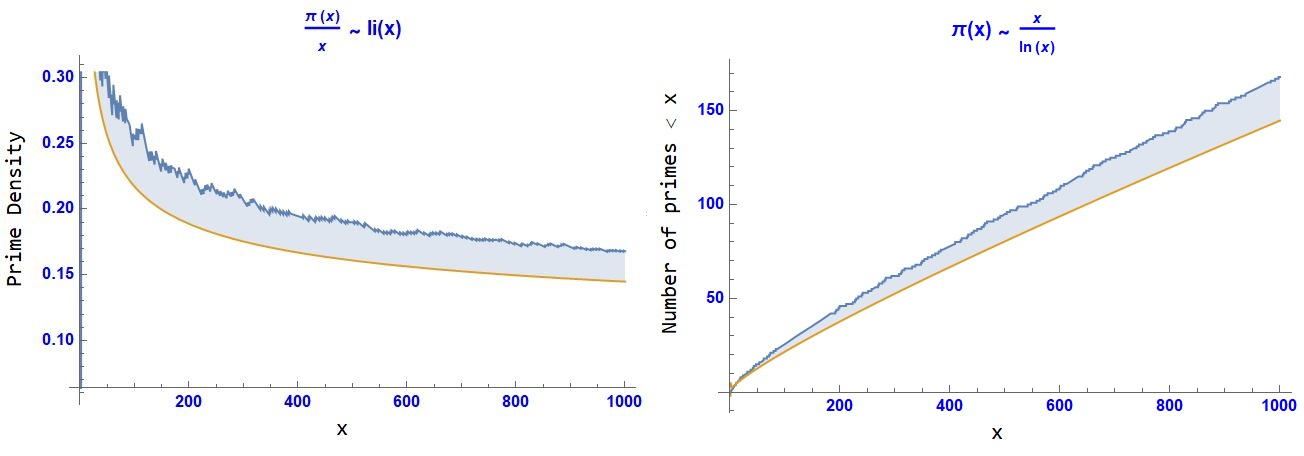
\includegraphics[scale=0.44]{images/fig1.JPG}
        % % figure caption is below the figure
        \caption{Demonstration of the Prime Number Theorem}
        \label{fig:1}       % Give a unique label
    \end{figure*}

\section{Proposed algorithm}
\label{sec:6}
The following is the algorithm underlying this cryptosystem
\begin{enumerate}
    \item \textbf{Encryption}
    \begin{enumerate}
        \item An input string (plain text) is taken and split into blocks, padding is applied. Padding is used to maintain consistency of the modified plain text. User provides the input string and block size.
        \item All characters in the blocks are converted to their corresponding ASCII values.
        \item In every block, every $i^{th}$ value is combined with the $(i+1)^{th}$ (adjacent) value using the \textit{Cantor pairing function}, which takes two numbers as input and spits back a single, unique number. Now, each block has $\left(\dfrac{\text{blocksize}}2\right)$ number of elements. Suppose the list is $$A=\left\{a_1,a_2,\cdots,a_{\text{blocksize}/2}\right\}$$
    \end{enumerate}
    \item \textbf{Key Generation}
    \begin{enumerate}
        \item \textit{The Chinese Remainder Theorem} requires that $$0<A_i<M_i$$ where $|A|=|M|=\dfrac{\text{block size}}{2}$. This key $M$ has to be generated. In order to ensure that this condition is met, the worst case scenario is considered where two characters with maximum ASCII value of $128$ appears adjacent to each other. For these two numbers, the Cantor pairing function returns $$C(128,128)=33024$$ All values of $M$ must be larger than $33024$, and an upper bound $U$ is also required so a finite loop can be run over this range $\left[\pi(128,128),N\right]$. $$C(128,128)\le M_i\le U\qquad \begin{cases} M=\left\{p_1,p_2,\cdots,p_n\right\},\forall p_i\in\text{Prime}\\|M|=N=\dfrac{\text{block size}}{2}\end{cases}$$
        \item This list of primes $M$ is shuffled and the solution to the following system of linear congruence equations generates the cipher text. $$x\equiv A_i\mod M_i$$
    \end{enumerate}
    \item \textbf{Decryption}
    \begin{enumerate}
        \item Cipher text $x$ and list of primes $M$ must be known for successful decryption. The solution to the following system of congruence equation is required $$A_i\equiv x\mod M_i$$
        \item Each $A_i$ is passed through the reverse cantor pair function to get back two adjacent $a_i$'s that initiated the encryption procedure.
        \item These $a_i$'s are converted to ASCII characters and padding sequences are removed.
    \end{enumerate}
\end{enumerate}

\section{Determining the upper bound}
\label{sec:7}
The prime number theorem gives us an estimate of the number of primes within a search size $x$. This asymptotic distribution is defined as $$\pi(x)\sim\dfrac{x}{\ln(x)}$$
\begin{enumerate}
    \item $\#$ of primes less than $n\implies\pi(n)\sim\dfrac{n}{\ln n}$
    \item $\#$ of primes in $(a,b)$$$\pi(b)-\pi(a)\sim\dfrac{b}{\ln b}-\dfrac{a}{\ln a}$$
    \item $\#$ of primes between $C(128,128)$ and an upper bound $U$ $$\pi(U)-\pi(C(128,128))\sim\dfrac{U}{\ln U}-\dfrac{C(128,128)}{\ln [C(128,128)]}$$
    \item It was stated in the algorithm that $N=\dfrac{\text{block size}}2$. This means
    
    \begin{align*}
        N&=\dfrac{U}{\ln U}-\underbrace{\dfrac{C(128,128)}{\ln [C(128,128)]}}_K\\N+K&=\dfrac{U}{\ln U}\\\ln U&=\dfrac{U}{N+K}\\
        \ln U&=\dfrac{U}{Q}\qquad\qquad where\quad Q=N+K\\
        U&=e^{\frac{U}{Q}}\\Ue^{-\frac{U}{Q}}&=1\\-\dfrac{U}{Q}e^{-\frac{U}{Q}}&=-\dfrac{1}{Q}\\-\dfrac{U}{Q}&=W_{-1}\left(-\dfrac{1}{Q}\right)\\
        U&=-QW_{-1}\left(-\dfrac{1}{Q}\right)\\&=-\left(N+\dfrac{C(128,128)}{\ln[C(128,128)]}\right)W_{-1}\left(-\dfrac{1}{N+\dfrac{C(128,128)}{\ln[C(128,128)]}}\right)
    \end{align*}
    where $W_n$ is the Lambert W Function\cite{corless1996lambertw,weisstein2002lambert} also known as the product log function. This means that it is possible to generate the upper limit for generating a list of primes for an arbitrary block size. Since the number of primes is positive, $U$ has to be positive so consequently $W_n\left(-\dfrac{1}{Q}\right)<0$. It means that the branch $n=-1$. If $U=a+ib$, i.e. $U\in\mathbb{C}$, considering $\operatorname{Re}(U)$ generates the upper limit. Let $x_1,x_2$ be the possible solutions after applying the Lambert W Function. Since $U>C(128,128)$, it can be safely assumed that $U=\max(x_1,x_2)$
\end{enumerate}
\FloatBarrier
\begin{flushleft}
Here is a table showing the initial number of values that has to be checked to generate a list of primes. Then, five primes are chosen at random, from this \textit{shuffled} list.
\end{flushleft}
% % For one-column wide figures use
% \begin{figure}
% % Use the relevant command to insert your figure file.
% % For example, with the graphicx package use
%   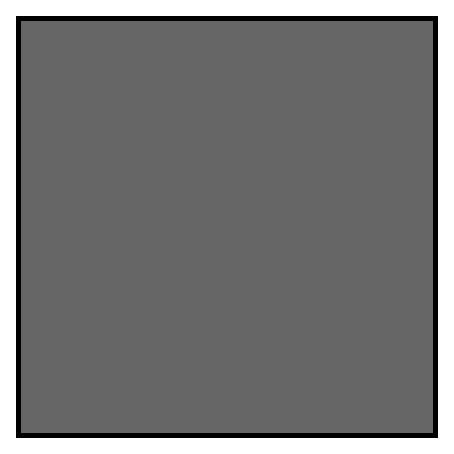
\includegraphics{example.eps}
% % figure caption is below the figure
% \caption{Please write your figure caption here}
% \label{fig:1}       % Give a unique label
% \end{figure}
% %
% % For two-column wide figures use
% \begin{figure*}
% % Use the relevant command to insert your figure file.
% % For example, with the graphicx package use
%   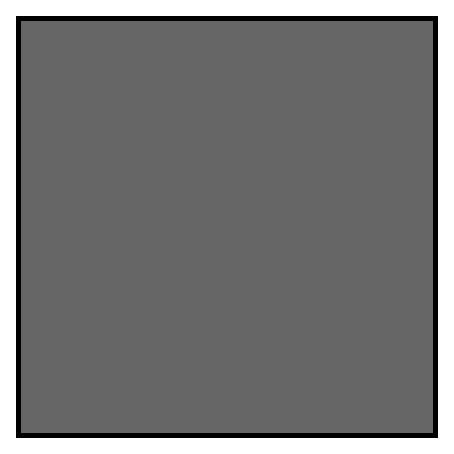
\includegraphics[width=0.75\textwidth]{example.eps}
% % figure caption is below the figure
% \caption{Please write your figure caption here}
% \label{fig:2}       % Give a unique label
% \end{figure*}
% %
% % For tables use
\begin{table}[htbp!]
% table caption is above the table
\caption{Block size and upper bound}
\label{tab:2}       % Give a unique label
\centering
% For LaTeX tables use
\begin{tabular}{l|cc|c|c}
\hline\noalign{\smallskip}
Block Size (bits) & $x_1$ & $x_2$ & $U=\max(x_1,x_2)$ & $U-C(128,128)$ \\
\noalign{\smallskip}\hline\noalign{\smallskip}
8	& 1.0003 & 33116 & 33116 & 730\\
16	& 1.0003 & 33208 & 33208 & 184\\
32	& 1.0003 & 33393 & 33393 & 369\\
64	& 1.0003 & 33761 & 33761 & 737\\
128	& 1.0003 & 34500 & 34500 & 1476\\
256	& 1.0003 & 35982 & 35982 & 2958\\
512	& 1.0003 & 38961 & 38961 & 5937\\
1024& 1.0002 & 44975 & 44975 & 11951\\
2048& 1.0002 & 57202 & 57202 & 24178\\
\noalign{\smallskip}\hline
\end{tabular}
\end{table}

\begin{flushleft}
Following is a plot showing the connection between the block size and the length of the range of numbers in which to look for primes. It is observed to demonstrate a fairly linear relationship.
\end{flushleft}
    \begin{figure*}[hbt!]
    \centering
        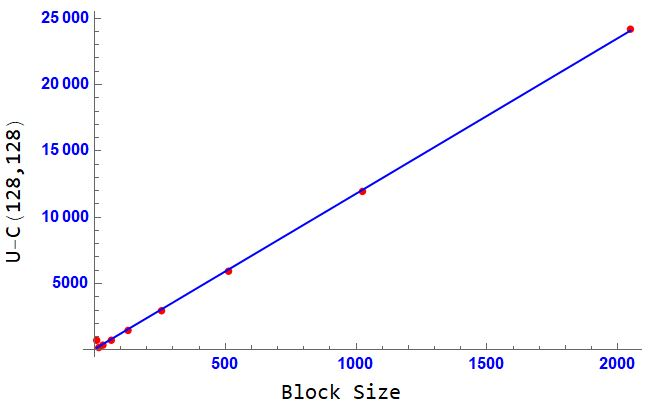
\includegraphics[scale=0.45]{images/fig2.JPG}
        % % figure caption is below the figure
        \caption{Block size vs prime search range}
        \label{fig:2}       % Give a unique label
    \end{figure*}

\section{Generating the list of primes}
\label{sec:8}
For the convenience of runtime complexity, an infinite loop was run from $C(128,128)$. The SymPy module in Python3 was used to generate primes adjacent to each other. The loop was terminated after the generation of $(\text{block size}/2)$ prime numbers. This method however, poses a serious problem. If an interceptor gets to know of this design, he/she would easily break the system using the classic \textit{Shor's Algorithm}.
On the other hand, if a set $S$ of randomly shuffled primes having sufficient gaps between each pair with cardinality of $(\text{block size}/2)$ is generated between $[C(128,128),U]$ where $U$ is the upper bound calculated in section \ref{sec:7}, then it would be quite tough for an interceptor to regenerate.

\section{From an interceptor's perspective}
\label{sec:9}
\subsection{Shor's Algorithm}
\label{subsec:9.1}
Shor's algorithm is a polynomial-time quantum computer algorithm for integer factorization \cite{365700}. Given a positive integer $$N=p_1^{k_1}p_2^{k_2}\cdots p_n^{k_n}$$, its job is to factor $N$ into its constituent prime factors and was innovated by Peter Shor in 1994. This can be achieved by using General Number Field Sieve with superpolynomial scaling: $O\left[\exp\left[c\left(\ln n\right)^\frac{1}{3}\left(\ln\ln n\right)^\frac{2}{3}\right]\right]$ where as Shor's runs only partially on a quantum computer, demonstrating a complexity of $O(\log n)^2(\log\log n)(\log\log\log n)$\cite{miszczak_2015}. This means an interceptor will not eventually have their way through the MES.
\subsection{Pollard's Rho Algorithm}
\label{subsec:9.2}
Pollard's rho algorithm is used for integer factorization. It was invented by John Pollard in 1975. \cite{pollard1974theorems} The algorithm is very fast for numbers with small factors, but slower in cases where all factors are large. The $\rho$. algorithm's most remarkable success was the factorization of the Fermat number $F_8$\cite{pollard1974theorems}. If the pseudorandom number $x=g(x)$ occurring in the Pollard $\rho$ algorithm were an actual random number, it would follow that success would be achieved half the time, by the Birthday paradox in $O({\sqrt{p}})\leq O(n^{1/4})$ iterations. It is believed that the same analysis applies as well to the actual rho algorithm, but this is a heuristic claim, and rigorous analysis of the algorithm remains open. \cite{galbraith201214} Since the primes chosen in the MES are sufficiently large it stops any unwelcome interceptor by raising the toughness of integer factorization while maintaining reasonable run time.

\section{Experimental analysis}
\label{sec:10}
A couple of benchmarking tests were performed to prove the worth and place of the proposed cryptosystem, among the already existing pool.

\subsection{String length vs Time for encrypt-decrypt cycle}
\label{subsec:10.1}
For this test, blocksize of $128,192$ and $256$ were considered and the length of string(with repetition) was gradually increased in steps of powers of $10$ while noting down the time it takes for successful encrypt-decrypt cycles.

%<Table comes here with 3 blocksize columns>
\begin{table}[htbp]
\caption{Effect of string length on run time for different block size}
\label{tab:3}
\centering
\begin{tabular}{|c|c|c|c|}
\hline
\multirow{2}{1.5cm}{String Length}& \multicolumn{3}{p{3cm}|}{\centering Block Size} \bigstrut \\
\cline{2-4} & \multicolumn{1}{c|}{128} & \multicolumn{1}{c|}{192} & \multicolumn{1}{c|}{256} \bigstrut \\ \hline
$10$ & $0.001$ & $0.002$ & $0.003$\bigstrut\\
$10^2$ & $0.002$ & $0.002$ & $0.002$\bigstrut\\
$10^3$ & $0.011$ & $0.012$ & $0.011$\bigstrut\\
$10^4$ & $0.13$ & $0.11$ & $0.115$\bigstrut\\
$10^5$ & $0.943$ & $1.053$ & $1.062$\bigstrut\\
$10^6$ & $9.807$ & $10.535$ & $11.106$\bigstrut\\
$10^7$ & $99.458$ & $106.824$ & $111.409$\bigstrut\\
\hline
\end{tabular}
\end{table}

\begin{flushleft}
It was observed that if the length of string is n and a $\text{block size}\gg n$ is used, then the time increases slightly owing to the excessive padding operation requirements.
\end{flushleft}

    \begin{figure*}[hbt!]
    \centering
        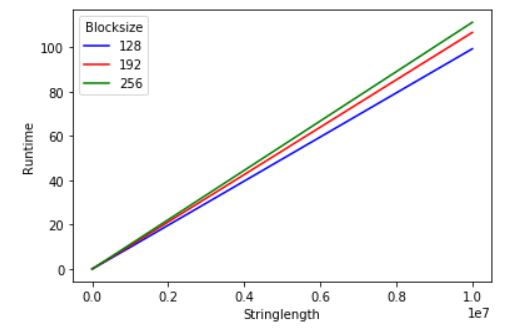
\includegraphics[scale=0.75]{images/fig3.JPG}
        % % figure caption is below the figure
        \caption{Block size vs run time}
        \label{fig:3}       % Give a unique label
    \end{figure*}
\FloatBarrier
\begin{flushleft}
In case $n\gg \text{block size}$, choosing a very small value for the block size vs choosing a comparatively larger block size leads to very similar time of execution but improved security in case of larger block size, thus making it all the more difficult for an interceptor to crack the message while ensuring reasonable run time complexity on the authorized pipeline.
\end{flushleft}

\subsection{Blocksize vs Time for encrypt-decrypt cycle}
\label{subsec:10.2}
A function was written on Jupyter Notebook to test out how varying the block size has an impact on the time it takes to complete one successful encryption-decryption cycle. Note that for this test, a random alphanumeric string of $26000$ characters was considered.

% % For tables use
\begin{table}[htbp!]
% table caption is above the table
\caption{Effect of block size on run time}
\label{tab:4}       % Give a unique label
% For LaTeX tables use
\centering
\begin{tabular}{lc}
\hline\noalign{\smallskip}
Block Size (bytes) & Run time (sec)\\
\noalign{\smallskip}\hline\noalign{\smallskip}
2	& 0.405\\
4	& 0.248\\
8	& 0.229\\
16	& 0.239\\
32	& 0.286\\
64	& 0.295\\
128	& 0.264\\
256	& 0.292\\
\noalign{\smallskip}\hline
\end{tabular}
\end{table}

\FloatBarrier
%\begin{flushleft}
Note that since every time the MES algorithm is executed, a unique secret key is generated depending on the block size. The bar and scatter plot in the first two images in Fig. \ref{fig:3} shows a fairly linear relationship with negligible slope when optimized. An \textit{ideal} system should resemble a horizontal line. This entropy in the real time is caused by multiple background processes that maybe running during the execution of this program.
%\end{flushleft}

    \begin{figure*}[hbt!]
    \centering
        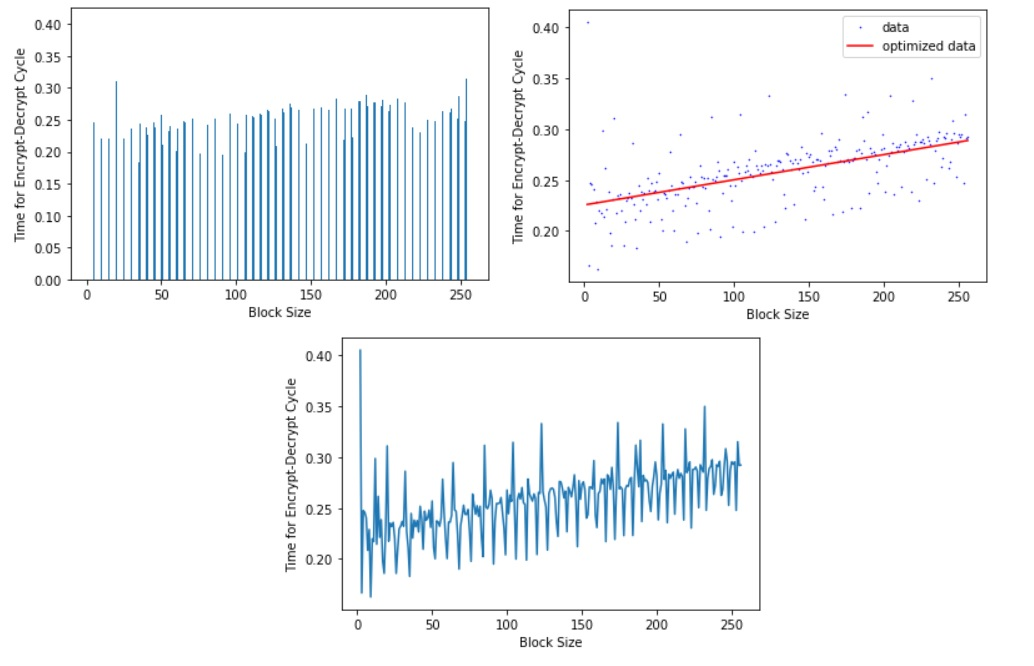
\includegraphics[scale=0.558]{images/fig4.jpg}
        % % figure caption is below the figure
        \caption{Block size vs run time}
        \label{fig:4}       % Give a unique label
    \end{figure*}

\section{Conclusion and Future Work}
\label{section: 11}
For benchmarking string length vs run time, $128,192$ and $256$ were taken as the block sizes in the experiment since AES also uses these bit length keys. However, it is crucial to note that AES and MES have a very different notion of block size and bit size. Unlike AES, the block size is not restricted to just $128,192,256$ in MES. Instead it can be any even positive integer chosen by the user. The idea of this paper was to introduce a new algorithm for future use. Since AES and DES involves bit wise calculations and MES simply works with ASCII values, there cannot be an effective comparison. However, if MES can somehow be converted into bits \cite{527526,chen2011efficient} and calculations involving byte substitution, bit shifting etc, are introduced, the run time should be much faster than AES and DES.

Use of ASCII values upfront is not the best approach for MES algorithm because it brings in computationally intensive task on the operations involved in the trapdoor function. However, if in future, the original message is converted into bits before applying MES then there would most likely be an exponential reduction in the complexity which can ultimately lead up to a great boost in performance of the algorithm to compete with industrially prevalent algorithms.

%\begin{acknowledgements}
%If you'd like to thank anyone, place your comments here
%and remove the percent signs.
%\end{acknowledgements}

% Authors must disclose all relationships or interests that 
% could have direct or potential influence or impart bias on 
% the work: 

\section*{Conflict of interest}
The authors declare that they have no conflict of interest.


% BibTeX users please use one of
%\bibliographystyle{spbasic}      % basic style, author-year citations
\bibliographystyle{spmpsci}      % mathematics and physical sciences
%\bibliographystyle{spphys}       % APS-like style for physics
\bibliography{References}   % name your BibTeX data base

% Non-BibTeX users please use
% \begin{thebibliography}{}
% %
% % and use \bibitem to create references. Consult the Instructions
% % for authors for reference list style.
% %
% \bibitem{RefJ}
% % Format for Journal Reference
% Author, Article title, Journal, Volume, page numbers (year)
% % Format for books
% \bibitem{RefB}
% Author, Book title, page numbers. Publisher, place (year)
% % etc
% \end{thebibliography}

\end{document}
% end of file template.tex